\documentclass[12pt,letterpaper]{article}
\usepackage{graphicx,textcomp}
\usepackage{natbib}
\usepackage{setspace}
\usepackage{fullpage}
\usepackage{color}
\usepackage[reqno]{amsmath}
\usepackage{amsthm}
\usepackage{fancyvrb}
\usepackage{amssymb,enumerate}
\usepackage[all]{xy}
\usepackage{endnotes}
\usepackage{lscape}
\newtheorem{com}{Comment}
\usepackage{float}
\usepackage{hyperref}
\newtheorem{lem} {Lemma}
\newtheorem{prop}{Proposition}
\newtheorem{thm}{Theorem}
\newtheorem{defn}{Definition}
\newtheorem{cor}{Corollary}
\newtheorem{obs}{Observation}
\usepackage[compact]{titlesec}
\usepackage{dcolumn}
\usepackage{tikz}
\usetikzlibrary{arrows}
\usepackage{multirow}
\usepackage{xcolor}
\newcolumntype{.}{D{.}{.}{-1}}
\newcolumntype{d}[1]{D{.}{.}{#1}}
\definecolor{light-gray}{gray}{0.65}
\usepackage{url}
\usepackage{listings}
\usepackage{color}

\definecolor{codegreen}{rgb}{0,0.6,0}
\definecolor{codegray}{rgb}{0.5,0.5,0.5}
\definecolor{codepurple}{rgb}{0.58,0,0.82}
\definecolor{backcolour}{rgb}{0.95,0.95,0.92}

\lstdefinestyle{mystyle}{
	backgroundcolor=\color{backcolour},   
	commentstyle=\color{codegreen},
	keywordstyle=\color{magenta},
	numberstyle=\tiny\color{codegray},
	stringstyle=\color{codepurple},
	basicstyle=\footnotesize,
	breakatwhitespace=false,         
	breaklines=true,                 
	captionpos=b,                    
	keepspaces=true,                 
	numbers=left,                    
	numbersep=5pt,                  
	showspaces=false,                
	showstringspaces=false,
	showtabs=false,                  
	tabsize=2
}
\lstset{style=mystyle}
\newcommand{\Sref}[1]{Section~\ref{#1}}
\newtheorem{hyp}{Hypothesis}

\title{Problem Set 1}
\date{Due: October 1, 2023}
\author{Applied Stats/Quant Methods 1}

\begin{document}
	\maketitle
	
	\section*{Instructions}
	\begin{itemize}
	\item Please show your work! You may lose points by simply writing in the answer. If the problem requires you to execute commands in \texttt{R}, please include the code you used to get your answers. Please also include the \texttt{.R} file that contains your code. If you are not sure if work needs to be shown for a particular problem, please ask.
\item Your homework should be submitted electronically on GitHub.
\item This problem set is due before 23:59 on Sunday October 1, 2023. No late assignments will be accepted.
\item Total available points for this homework is 80.
	\end{itemize}
	
	\vspace{1cm}
	\section*{Question 1 (40 points): Education}

A school counselor was curious about the average of IQ of the students in her school and took a random sample of 25 students' IQ scores. The following is the data set:\\
\vspace{.5cm}

\lstinputlisting[language=R, firstline=36, lastline=36]{PS01_AF.R}  

\vspace{1cm}

\begin{enumerate}
	\item Find a 90\% confidence interval for the average student IQ in the school.\\
	

		
	My answers
	
	In order to get the Confidence Interval for population mean (CI), we have to understand the formula and its elements
	To get the Standard Error (SE), we need the Standard Deviation (S) and to get the S we need to get the Variance ($S^2$)
	The first thing I did, it was to answer this problem set on paper \& using Excel, you will find a copy of the Excel file in the same folder
	Second learn the commands in R and corroborate the results
	To get the $S^2$ we need to know the Sample Size (n), Y1,Y2,...Yn (Observations) and the Y (Sample mean)
	Note: sometimes we find X instead of Y in the formula that does not matter
	
	To calculate the mean we just have to use the following command: mean(y)
	We previously said y is our universe of observations I will put the \# of row here
	
	To get the formula of the variance done we just have to type var(y)
	Actually we could have jumped into Variance but is useful to have, we don't have to do it by parts but is useful to visualize the mean and n. Also we will need both for our final formula CI
	
	To get the Standard Error we need to follow the formula SE=S/square n
	As we already know the value of S = Standard Deviation = 13.09 and the value of n = 25, we just have to replace and follow the next command: 	sd(y)/sqrt(25)
	
	At this point we have all the values needed to answer the formula of CI
	$CI=X+-Z S/\sqrt(n)$
	Confidence Interval=Sample mean +-Zscore*Standard deviation /square sample size
	There are two important things about this in this case X with a hat is 
	the sample mean, as previously said some author represent it with y an a hat
	2nd the Zscore we were told to find a 90\% CI
	
	We are 90\% confident that if we pick a random sample, the average student IQ in that school we fall between 93.46 and 103.42
	

	
	\item Next, the school counselor was curious  whether  the average student IQ in her school is higher than the average IQ score (100) among all the schools in the country.\\ 
	
	\noindent Using the same sample, conduct the appropriate hypothesis test with $\alpha=0.05$.
\end{enumerate}

\begin{verbatim}
	Hypothesis test a = 0.05
	Ho Null Hypothesis, Ho=100
	Ha Alternative Hypothesis, Ha dif 100
	
	P-value = 0.5569, usually P<=0.05 "statistically significant" result
	Smaller P-Values more strongly contradict the null.
	For this exercise I will not take in consideration P as our n is too small.
	
	We reject our Null Hypothesis as our Ho is not equal to 100 as we specified in our hypothesis. 


\end{verbatim}

\newpage

	\section*{Question 2 (40 points): Political Economy}

\noindent Researchers are curious about what affects the amount of money communities spend on addressing homelessness. The following variables constitute our data set about social welfare expenditures in the USA. \\
\vspace{.5cm}


\begin{tabular}{r|l}
	\texttt{State} &\emph{50 states in US} \\
	\texttt{Y} & \emph{per capita expenditure on shelters/housing assistance in state}\\
	\texttt{X1} &\emph{per capita personal income in state} \\
	\texttt{X2} &  \emph{Number of residents per 100,000 that are "financially insecure" in state}\\
	\texttt{X3} &  \emph{Number of people per thousand residing in urban areas in state} \\
	\texttt{Region} &  \emph{1=Northeast, 2= North Central, 3= South, 4=West} \\
\end{tabular}

\vspace{.5cm}
\noindent Explore the \texttt{expenditure} data set and import data into \texttt{R}.
\vspace{.5cm}
\lstinputlisting[language=R, firstline=54, lastline=54]{PS01_AF.R}  
\vspace{.5cm}


	My answers
	Import data into R:
	First thing is to transform the file into a .CSV, we just have to rename the file, second thing is to bring our file into R, we can do this using a code and adding the location of our file, or we can use our right-down window with the option Import Text Data. Doing the second option we have to change the Delimeter to "Tab" as the columns in our .CSV file are separated by space, then R will recognize the columns/variables in our file instead of bringing just one. In our right side we will have the code that R is going to apply, so next time we can use that lines instead of the option Import Text Data. We press import to confirm the action. 
	Note: I changed the first letter for a capital letter in the name of the file.
	
	Explore the data set
	I run some codes in R to explore the data set such as: str, glimpse, dim, lenght, View, head, tail, etc.
	Note: It is important to run the line library tidyverse to be able to use glimpse and other functions. 
	
	The first two give us an idea of the structure of our data, what type of variables we have, character, numeric, list, etc.
	The rest is to understand our number of observations and variable we have, I personally like the head function because I don't have to change of tab to visualize my data and I can get an idea of what we are analysing. 
	
	One thing that I noticed while analysing our data set is that we don't have missing information or N/A in our data, which is good for our analysis
	
	In the second part I rename our columns/variables for names I find easier to remember. Finally I use the code summary for each column to have an idea of the minimum, maximum, mean, media, etc. of each variable. 	
	


\begin{itemize}
\item
Please plot the relationships among \emph{Y}, \emph{X1}, \emph{X2}, and \emph{X3}? What are the correlations among them (you just need to describe the graph and the relationships among them)?
\vspace{.5cm}


	Answer A:
	Y and X1 = Answer can be seen on option C
	Y and X2 = Expenditure on shelters/housing assistance vs number of residents financially insecure in state.
	First thing I ran a few commands; hist, mean, var, sd, standard error, the ones using in Question 1 of this problem set. I did it on each one to get a general understanding on Y and X2. Once I did this I ran the commands cor and plot, I got 0.45 on correlation, this is a positive but not a strong correlation, still both variables move in the same direction, and from the graph I can see a slight curve, start with a high expenditure on residents financially insecure, while we move to the center the expenditure decrease and finally finish going higher than the start. 
	
	\begin{figure}[h!]\centering
		\caption{\footnotesize Boxplot of $Y$ by $Region$.}\vspace{-1cm}
		\label{fig:plot_3c}
		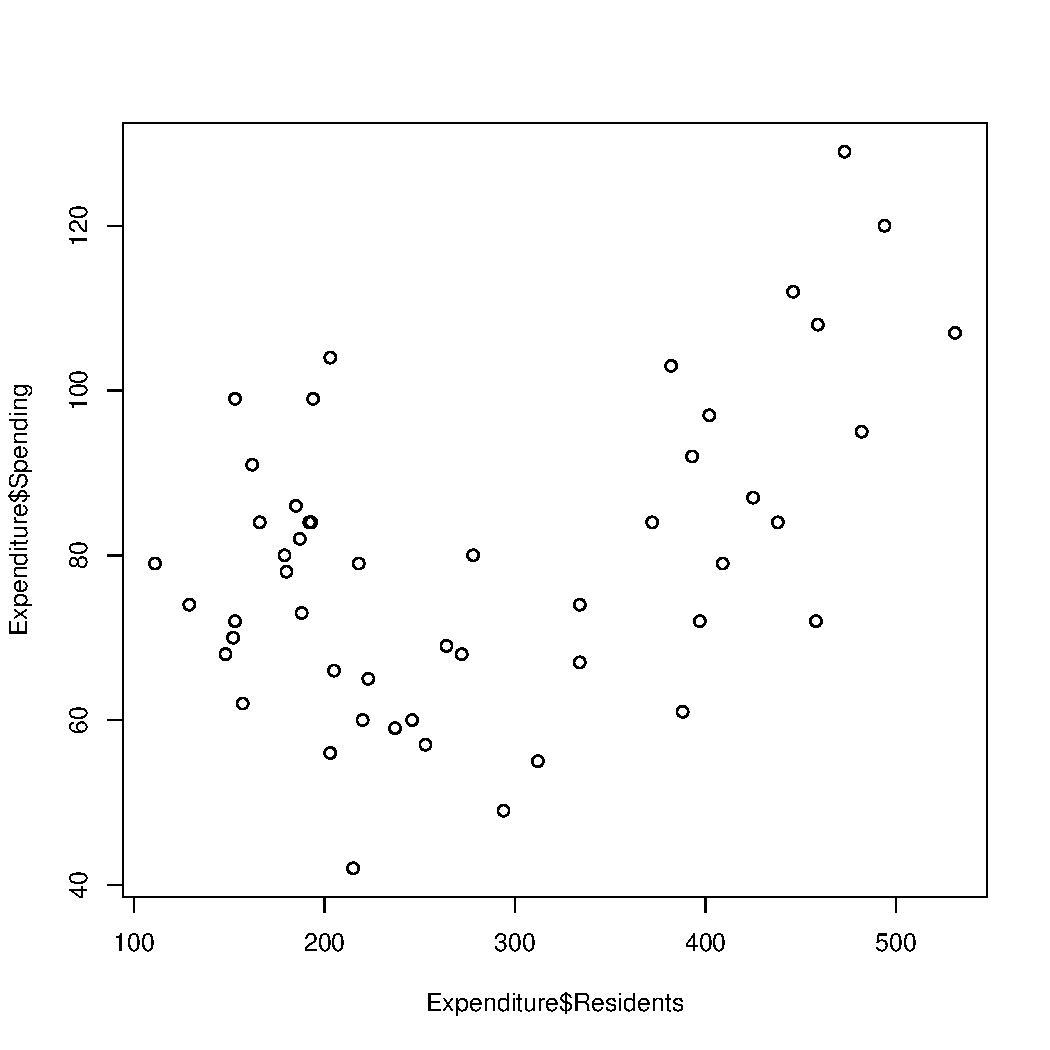
\includegraphics[width=.75\textwidth]{IMAGEP2_A.pdf}
	\end{figure}
	
	Y and X3 = Expenditure on shelters/housing assistance vs number of people residing in urban areas in state.
	I reply the step and use the same commands than before, I am specially interested in the hist to see the distribution, I got 0.46 on correlation, a similar number than before and that suggest the same, a moderate positive correlation between the two variables, when the expenditure increase our variable does it as well, so more people residing in urban areas. In this case, on the graph we can see a linear movement slightly increasing when we move from left to right. Which suggest that the expenditure increase when people lives on urban areas. That can be because people on cities tends to have better income, and the government focus on the ones with less money.
	
	\begin{figure}[h!]\centering
		\caption{\footnotesize Boxplot of $Y$ by $Region$.}\vspace{-1cm}
		\label{fig:plot_3c}
		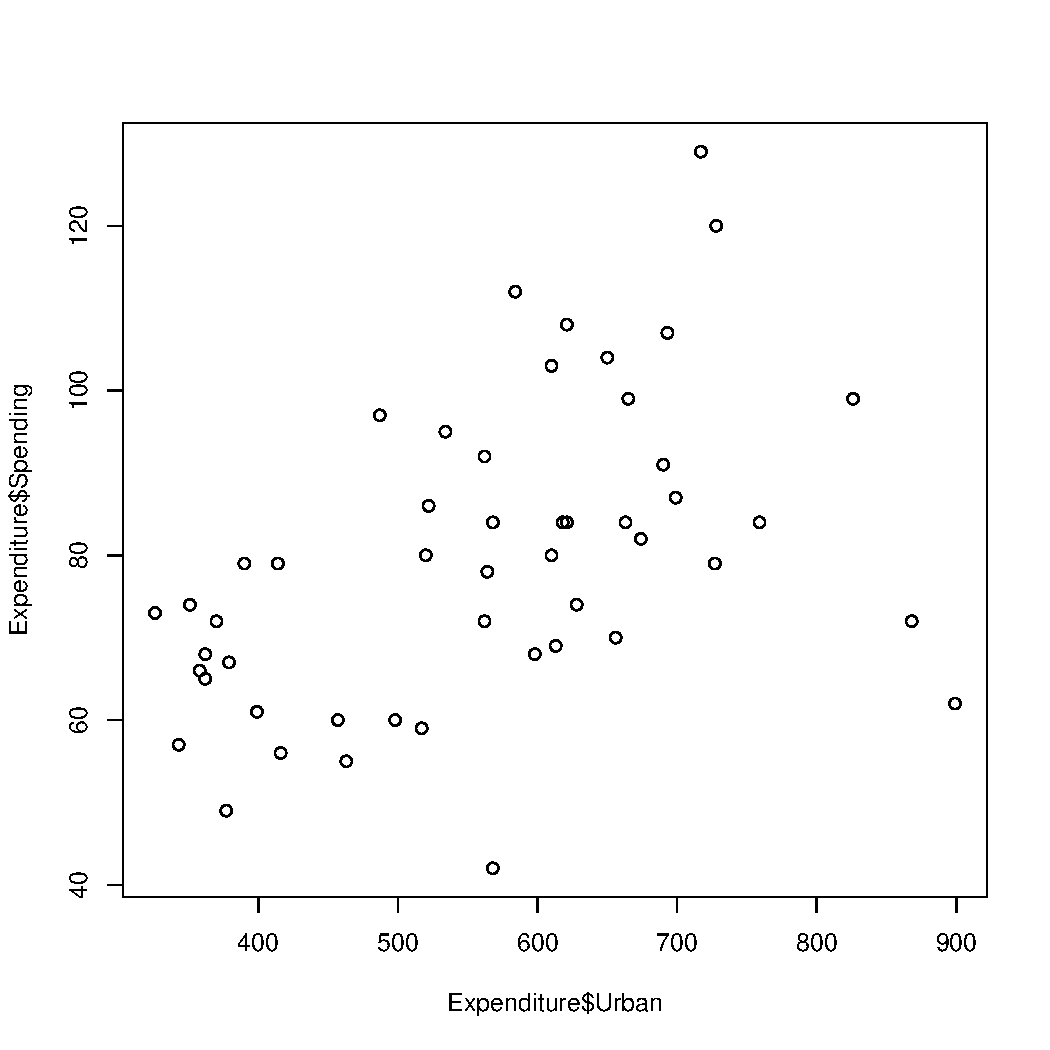
\includegraphics[width=.75\textwidth]{IMAGEP2_A1.pdf}
	\end{figure}
	
	X1 and X3
	To corroborate the last assumption I decided to compare my variable X1 Income vs X3 People in Urban areas.
	Here I am using X1 and my dependent variable Y
	The correlation is 0.59, which indicate that as one variable increase the other tends to increase as well, and I can see that from the graph the income increase when people lives further from Urban areas. 
	
	
	\begin{figure}[h!]\centering
		\caption{\footnotesize Boxplot of $Y$ by $Region$.}\vspace{-1cm}
		\label{fig:plot_3c}
		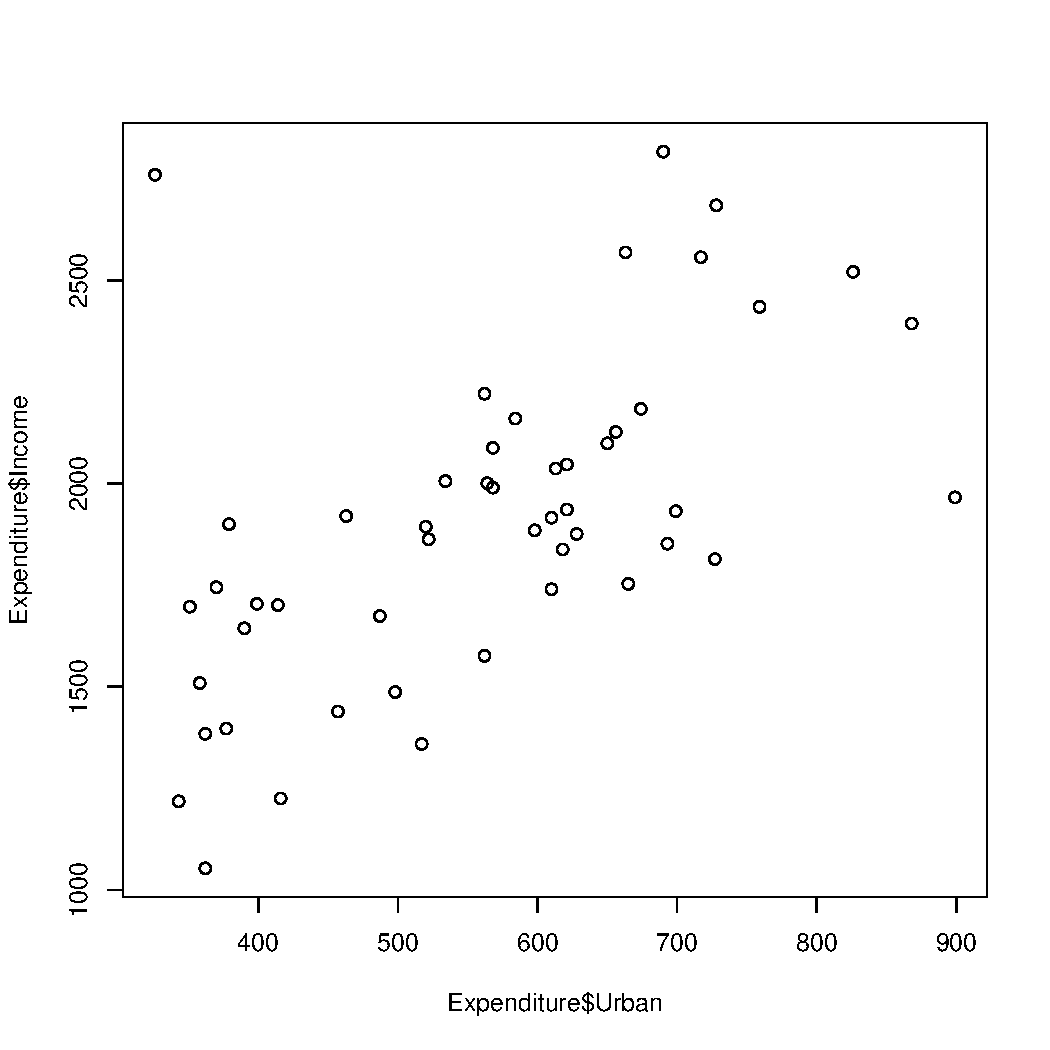
\includegraphics[width=.75\textwidth]{IMAGEP2_A2.pdf}
	\end{figure}
	
	X2 and X3
	For curiosity I plot variable 2 and variable 3, thinking that the number of residents financially insecure in state X2, could be concentrate on people living in urban areas. However I got a correlation of 0.22 which is low and I cannot see anything on the graph that suggest it is true. 
	
	Note: a correlation does not imply causation.

\begin{figure}[h!]\centering
	\caption{\footnotesize Boxplot of $Y$ by $Region$.}\vspace{-1cm}
	\label{fig:plot_3c}
	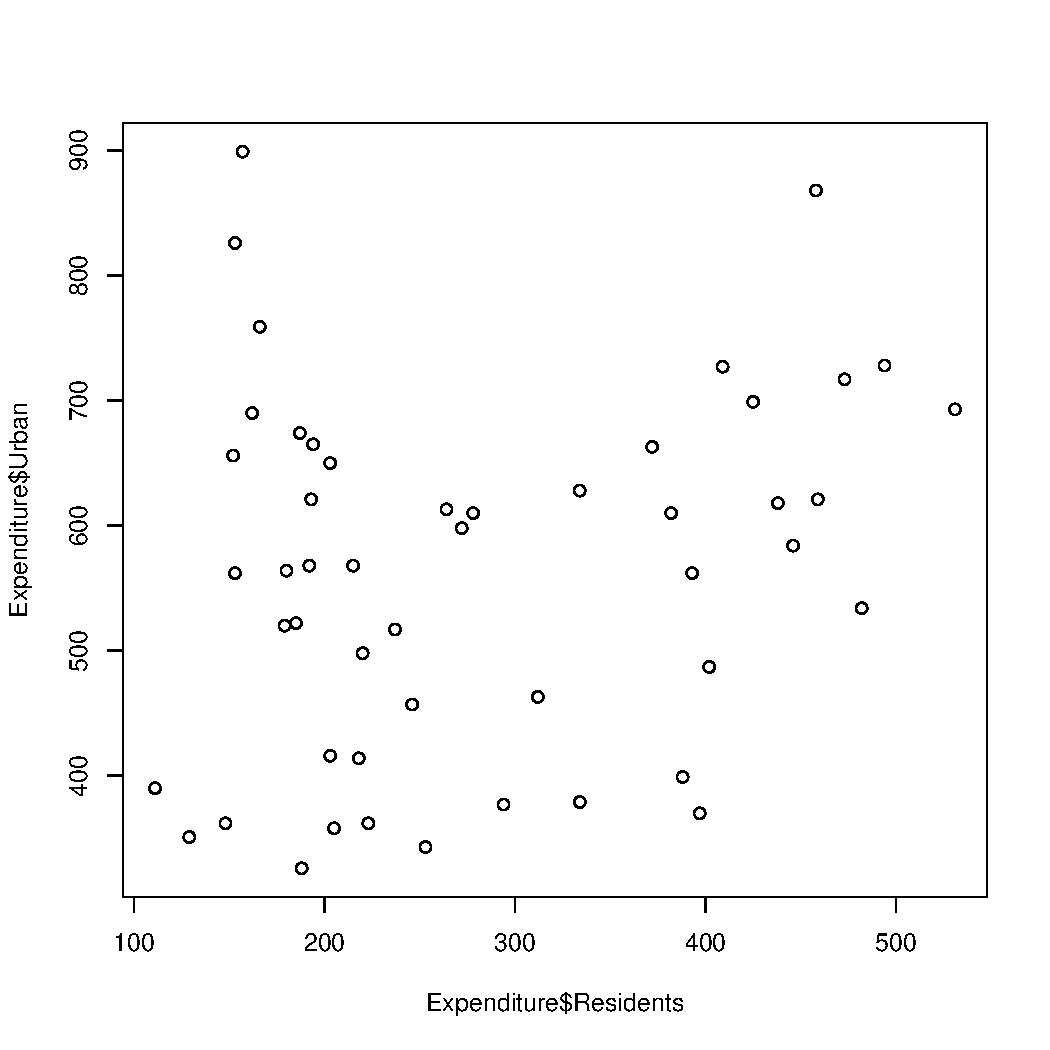
\includegraphics[width=.75\textwidth]{IMAGEP2_A3.pdf}
\end{figure}


\item
Please plot the relationship between \emph{Y} and \emph{Region}? On average, which region has the highest per capita expenditure on housing assistance?
\vspace{.5cm}


	
	Answer B:
	Y and Region = Relationship between Y (Spending=Expenditure) and Region
	There is no positive or negative correlation between Expenditure and Region 0.06
	In our graph we can see that the distribution is different between the sample taken on each region i.e. Region number 2 and Region number 4
	It seems from the graph that Region 4 = West, has the highest per capita expenditure on housing assistance.
	
	\begin{figure}[h!]\centering
		\caption{\footnotesize Boxplot of $Y$ by $Region$.}\vspace{-1cm}
		\label{fig:plot_3c}
		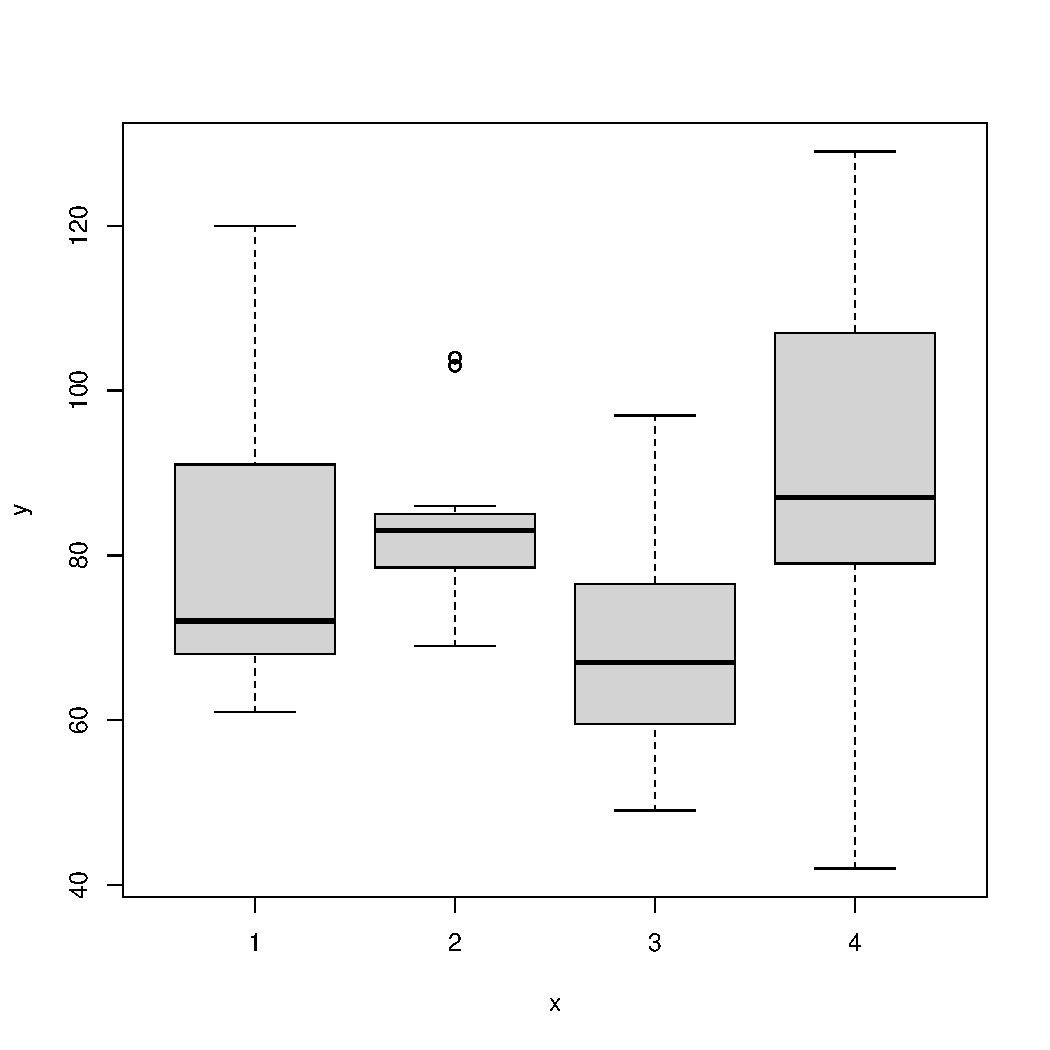
\includegraphics[width=.75\textwidth]{IMAGEP2_B1.pdf}
	\end{figure}
	
	For this case I use a new command ggplot, same I used on option C to visualize the data. However from both graphs can be visualised that region 4 has the highest per capita expenditure on housing assistance. 
	I decided to test this, finding the average of each region, for this I use Excel, being the results; Region 1 = 79.44, Region 2 = 83.92, Region 3 = 69.19 and Region 4 = 88.3.
	So Region 4 is on average the region with the highest per capita expenditure on housing assistance. 

\begin{figure}[h!]\centering
	\caption{\footnotesize Boxplot of $Y$ by $Region$.}\vspace{-1cm}
	\label{fig:plot_3c}
	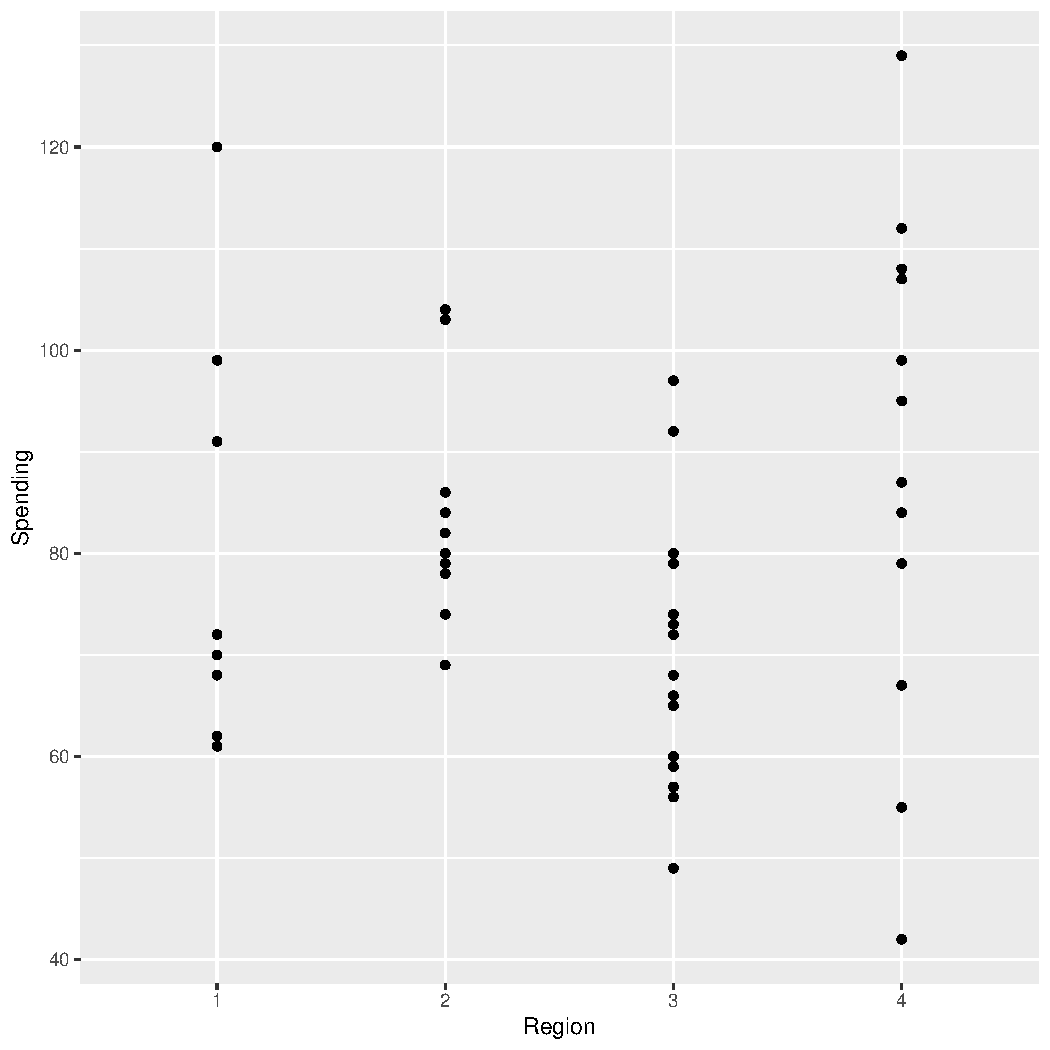
\includegraphics[width=.75\textwidth]{IMAGEP2_B2.pdf}
\end{figure}




\item
Please plot the relationship between \emph{Y} and \emph{X1}? Describe this graph and the relationship. Reproduce the above graph including one more variable \emph{Region} and display different regions with different types of symbols and colors.
\end{itemize}


	
	Answer C:
	Relationship between Y Spending and X1 Income
	There is a positive correlation 0.53 between the income and the spending/expenditure, the relationship appears to be positive: If the income is higher The expenditure on shelters/housing assistance increase.
	I ran the common codes; hist, mean, var, sd, etc. But in order to add symbols and colors I had to use additional codes on my graph. The exercise of the penguins on the book R for Data Science, 2 Data Visualization gives a very clear idea on how to construct our graph from scratch using the following codes: ggplot, geom\_point, geom\_smooth, aes, color, and shape.
	As I was not getting the colors and the shapes I had to use the code scale\_shape\_manual and type the colors I want to use, I did the same for shapes scale\_shape\_manual and type the figures I wanted in my graph. 
	Note: It is important to run the code library ggplot2, otherwise some of the functions won't work.
	 

\begin{figure}[h!]\centering
	\caption{\footnotesize Boxplot of $Y$ by $Region$.}\vspace{-1cm}
	\label{fig:plot_3c}
	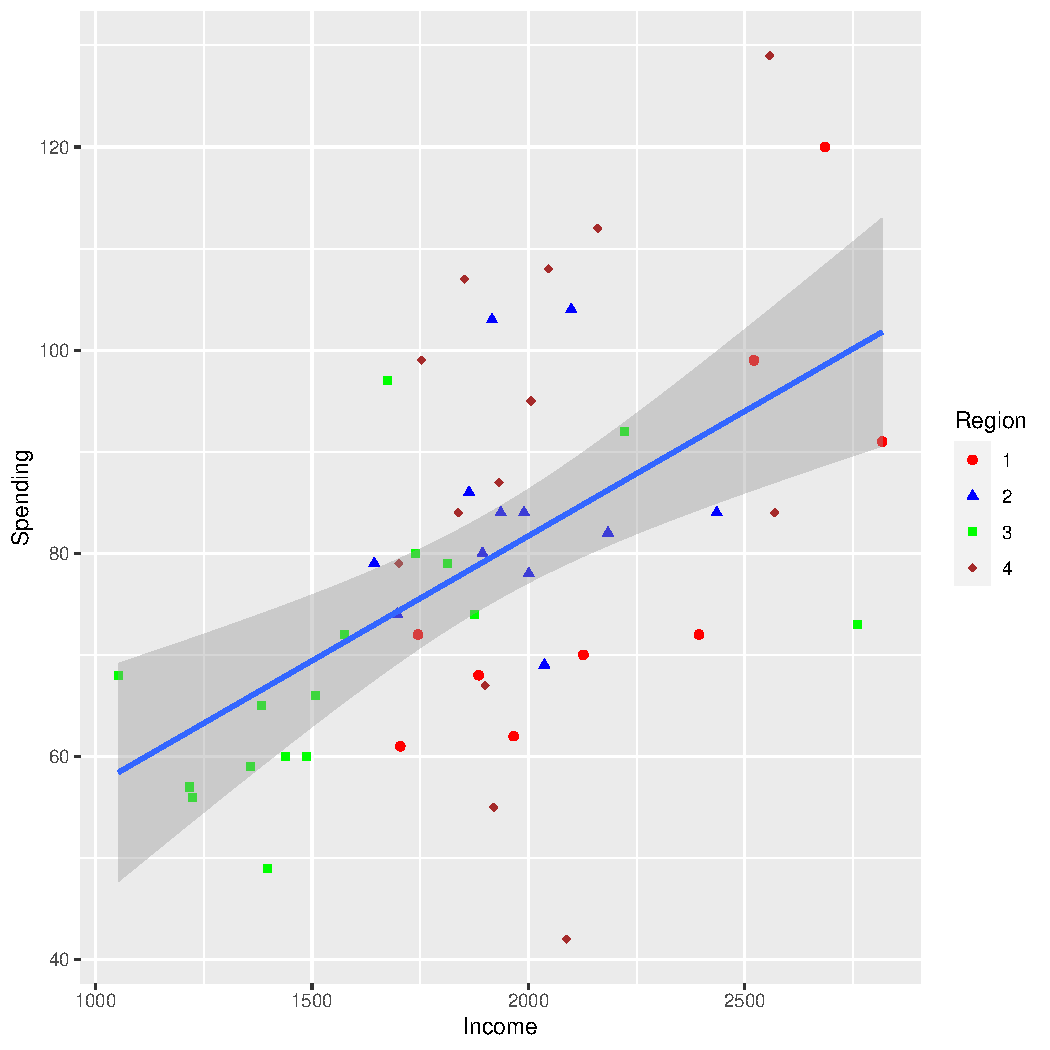
\includegraphics[width=.75\textwidth]{IMAGEP2_C.pdf}
\end{figure}

\end{document}
